\chapter{Goals}

Aside from fossils, the trace element chemistry of sediments can provide
strong indications of facies and salinity at the time of deposition.
Wet-chemistry based methods for determining trace element contents in rock samples
are labour-intensive, and often have large uncertainties~\parencite{bowen-sr-1956}.
Instrumental techniques, for example X-ray fluorescence (\acronym{XRF}) or mass spectrometry, 
are often more accurate. Many are also straightforward to use, and allow the rapid analysis of many 
samples~\parencite{ichikawa-xrf-2016,he_rapid_2018, he_determination_2019}.
This work will investigate the use of trace element ratios to characterize clay-rich 
sediments proposed by \textcite{Worden_1996} and \textcite{wei-2020} on sediments 
from the \acronym{UMM} and \acronym{USM} using instrumental methods. 
Because these sediments were deposited in a marginal setting where the foreland basin
quickly filled with terrigenous sediment,
it is unclear if the results from \textcite{Worden_1996} and \textcite{wei-2020} carry 
over to this setting.

As examples, sediments from the area around the village of 
Vorderthal in Switzerland (\cref{fig:study_area}) will be used.
The location is at the Alpine front, where the molasse sediments overlay sediments of 
the Helvetic nappe and are intensely folded (cf. \cref{fig:molasse_profile}).

\begin{figure}
\centering
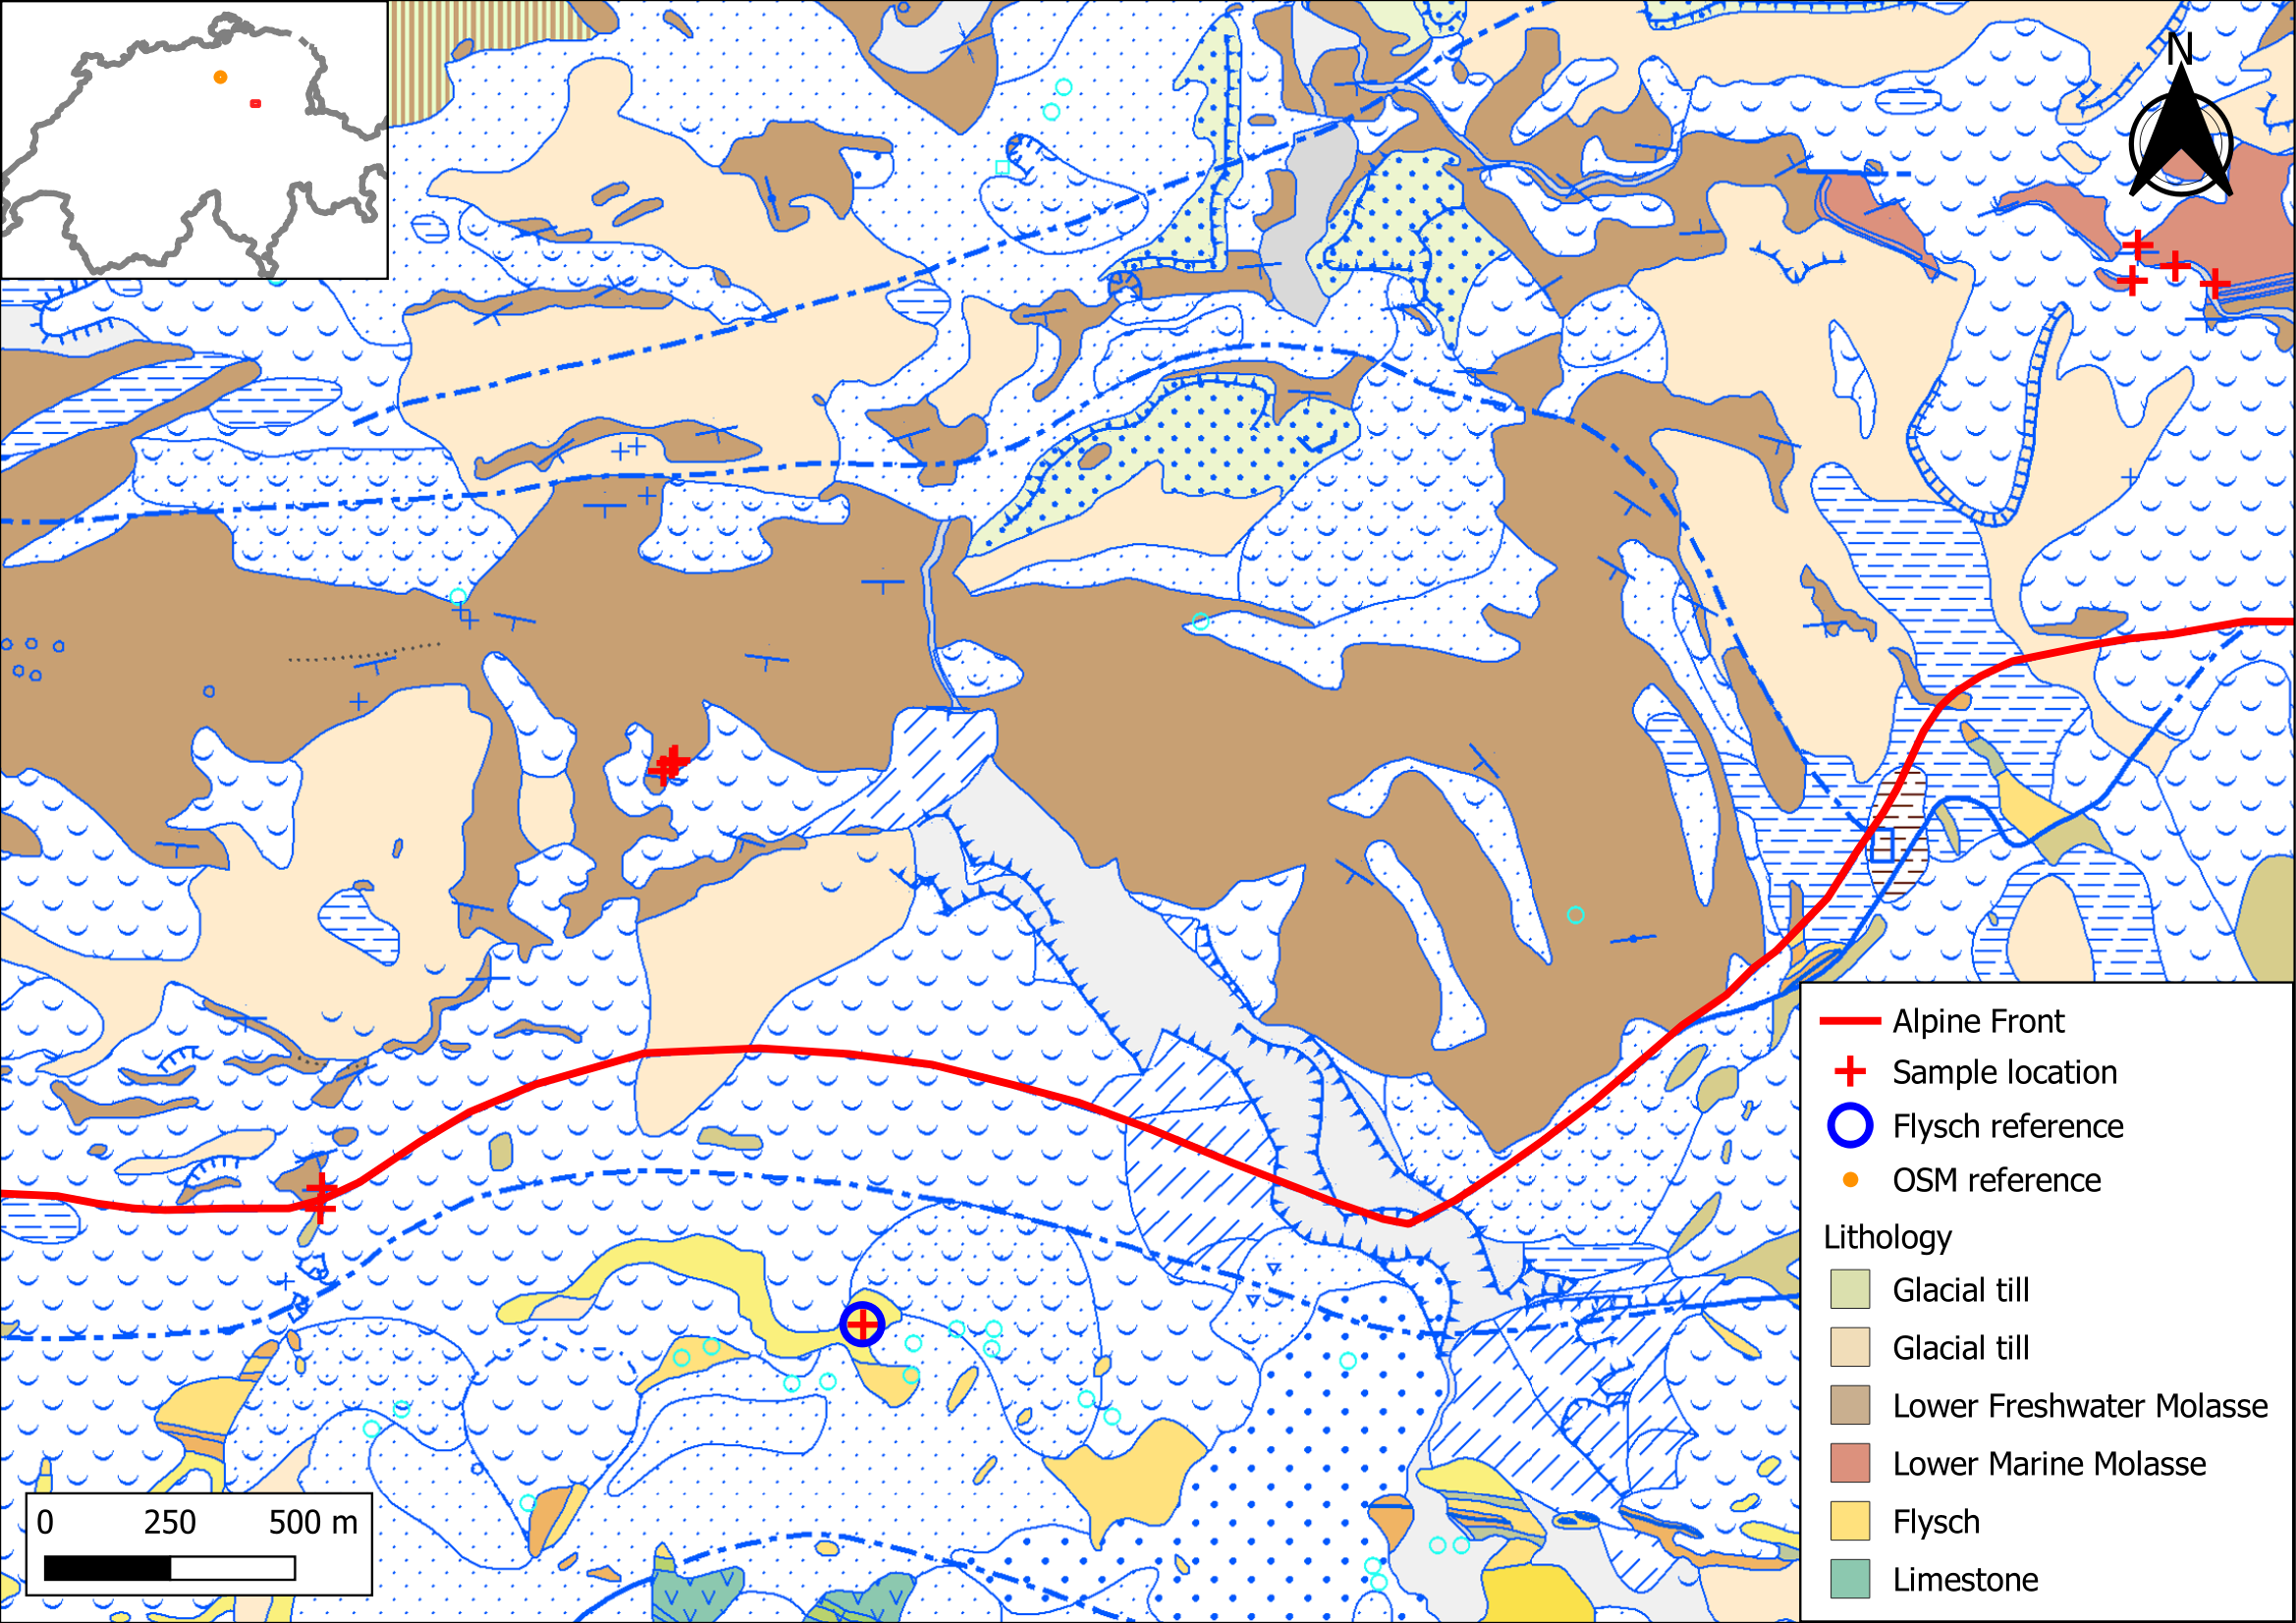
\includegraphics[width=.95\textwidth]{img/study_area.png}
\caption{The study area with sample locations. The OSM reference location is at the blue
dot in the overview insert.
Modified from \citeauthor{swisstopo}.}\label{fig:study_area}
\end{figure}

The \textbf{primary goal} of this work is to classify a number of rock samples into
marine and terrestrial sediments using instrumental methods. 
The experiments will:
\begin{itemize}
    \item Test whether \citeauthor{Worden_1996}'s \citeyear{Worden_1996} method 
    using the \acronym{Cl}/\acronym{Br} ratio is sufficient for a full classification.
    \item Test if the linear relationships for the \acronym{Sr}/\acronym{Ba}, 
    \acronym{Cl}/\acronym{Br} and \acronym{S}/\acronym{TOC} ratios determining the 
    fresh, brackish and marine
    water distinction established by \textcite{wei-2020} holds for our samples.
    \item Validate and if necessary update the geological map of the study 
    area~(\cref{fig:study_area}), if additional
    methods are not needed or quick enough to apply.
\end{itemize}